\section{Complete Block Designs}

In many situations we know that our experimental units are not homogeneous. Making explicit use of the special structure of the experimental units typically helps reduce variance. We apply the treatments to the same object / subject. This makes the subject-to-subject variability completely disappear. We also say that we block on subjects or that an individual subject is a block.
\begin{center}
	\includegraphics[width=0.8\linewidth]{block-illustration.png}
\end{center}


\subsection{Randomized Complete Block Designs}

Assume that we can divide our experimental units into $r$ groups, also known as blocks, containing $g$ experimental units each. The \textbf{randomized complete block design} (RCBD) uses a restricted randomization scheme: Within every block, the $g$ treatments are randomized to the $g$ experimental units. The design is called \textbf{complete} because we observe the complete set of treatments within every block. Note that blocking is a special way to design an experiment, or a special "flavor" of randomization. It is not something that you use only when analyzing the data.\medskip

The experimental units should be as similar as possible within the same block, but can be very different between different blocks. This design allows us to fully remove the between-block variability from the response because it can be explained by the block factor. In that sense, blocking is a so-called variance reduction technique. The randomization step within each block makes sure that we are protected from unknown confounding variables. Typcial block factors are location, day, machine operator, subjects, etc. \medskip

In the most basic form, we assume that we do not have replicates within a block. This means that we only observe every treatment once in each block. The analysis of a randomized complete block design is straightforward. We treat the block factor as "just another" factor in our model. As we have no replicates within blocks, we can only fit a\textbf{ main effects model} of the form:
$$Y_{ij} = \mu + \alpha_i + \beta_j + \epsilon_{ij}$$

We implicitly assume that blocks only cause additive shifts. Or in other words, the treatment effects are always the same, no matter what block we consider.\medskip

Typically, we are not inspecting the $p$-value of the block factor, mainly because of the fact that we did not randomize blocks to experimental units and we already knew that blocks are different. We would like the block factor to explain a lot of variation, hence if the mean square of the block factor is larger than the error mean square $MS_E$ we conclude that blocking was efficient. \medskip

Instead of a single treatment factor we can also have a factorial treatment structure within every block, e.g. a two-factor factorial which we would model as $Y \sim Block + A * B$. Here, we could actually test the interaction between $A$ and $B$ even if every level combination appears only once in every block. As we have multiple blocks, we have multiple observations for every level combination of $A$ and $B$! However, a randomized complete block design can only be used with one blocking factor.

\begin{center}
	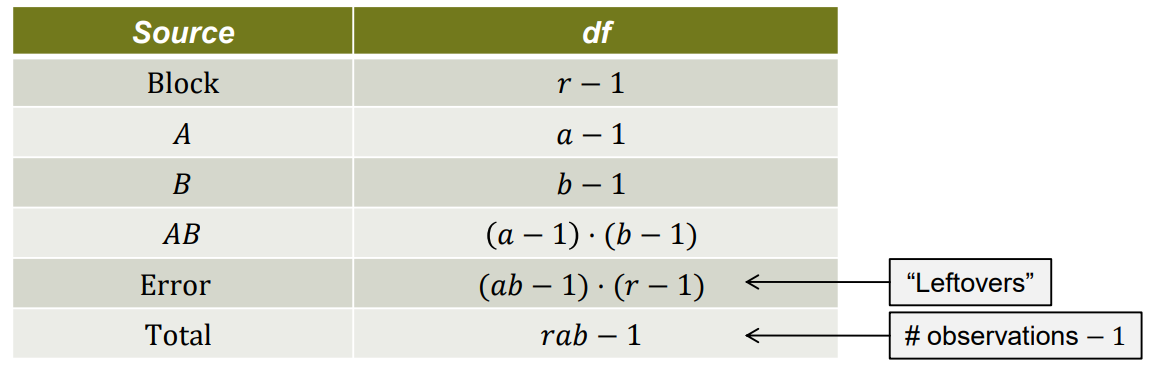
\includegraphics[width=\linewidth]{df_two-factor_factorial.png}
\end{center}

We can test for interactions even if we only have one replicate per combination and block.

\subsection{Multiple Block Factors}

We can also block on more than one factor. A special case is the so-called \textbf{Latin Square design} where we have two block factors and one treatment factor having $g$ levels each. Hence, this is a very restrictive assumption. \medskip

In a Latin Square design, each treatment appears exactly once in each row and once in each column. A Latin Square design blocks on both rows and columns simultaneously. We also say it is a \textbf{row-column design}.
\begin{center}
	\begin{tabular}{c c c c c}
		 & $C_1$ & $C_2$ & $C_3$ & $C_4$\\ \hline
		 $R_1$ & A & B & C & D \\ \hline
		 $R_2$ & B & A & D & C \\ \hline
		 $R_3$ & C & D & A & B \\ \hline
		 $R_4$ & D & C & B & A \\ \hline
	\end{tabular}
\end{center}

To analyze data from such a design, we use the main effects model:
$$Y_{ijk} = \mu + \alpha_i + \beta_j + \gamma_k + \epsilon_{ijk}$$

The design is balanced having the effect that our usual estimators and sums of squares are "working". In R, we would use the model formula \textit{y $\sim$ Block1 + Block2 + Treat}. We cannot fit a more complex model, including interaction effects, here because we do not have the corresponding replicates.

\subsubsection{Graeco-Latin Squares}

If we have another blocking criterion with $g$ levels (denoted by Greek letters, e.g. with levels $\alpha, \beta, \gamma, \delta$), we can use a Graeco-Latin Squares design. The conditions are that the Latin letters (treatments) occur once in each row and column and the Greek letters (third block factor) occur once in each row and column, i.e. we have two superimposed Latin Squares. In addition, each Latin letter occurs exactly once with each Greek letter. We use the main effects model to analyze the data:
$$Y_{ijkl} = \mu + \alpha_i + \beta_j + \gamma_k + \delta_l + \epsilon_{ijkl}$$

Where $\alpha_i$ is the treatment, $\beta_j$ the block factor 1, $\gamma_k$ the block factor 2 and $\delta_l$ the block factor 3. 

\begin{center}
	\begin{tabular}{c c c c c}
		 & $C_1$ & $C_2$ & $C_3$ & $C_4$\\ \hline
		 $R_1$ & A$\alpha$ & B$\gamma$ & C$\delta$ & D$\beta$ \\ \hline
		 $R_2$ & B$\beta$ & A$\delta$ & D$\gamma$ & C$\alpha$ \\ \hline
		 $R_3$ & C$\gamma$ & D$\alpha$ & A$\beta$ & B$\delta$ \\ \hline
		 $R_4$ & D$\delta$ & C$\beta$ & B$\alpha$ & A$\gamma$ \\ \hline
	\end{tabular}
\end{center}


\subsection{Precision}

In a RCB design, the squared standard errors are $\frac{\sigma_{RCB}^2}{r}$, where $r$ is the number of blocks, and in a completely randomized design $\frac{\sigma_{CRD}^2}{n}$. If we want to have the same precision, we need to ensure that:
$$\frac{\sigma_{RCB}^2}{r} = \frac{\sigma_{CRD}^2}{n}$$

Therefore, if we knew both squared standard errors, we would have to use a ratio of $\frac{n}{r} = \frac{\sigma_{CRD}^2}{\sigma_{RCB}^2}$. \medskip

$\sigma_{RCB}^2$ is estimated by the $MS_E$ of our RCB and $\sigma_{CRD}^2$ can be estimated using a weighted average of $MS_E$ and $MS_{Block}$. The relative efficiency is then defined as:
$$RE = \frac{\hat \sigma_{CRD}^2}{\hat \sigma_{RCB}^2}$$

And gives us the ratio $n / r$, which can be interpreted as how many experimental units would be needed by a CRD to achieve the same efficiency / precision. Easier for a quick check is to look at the ratio $MS_{Block} / MS_E$, because:
$$\frac{MS_{Block}}{MS_E} > 1 \; \Leftrightarrow \; RE > 1$$
